%\documentclass[a4paper, 12pt]{scrreprt}

\documentclass[a4paper, 12pt]{scrartcl}
%usepackage[german]{babel}
\usepackage{microtype}
%\usepackage{amsmath}
%usepackage{color}
\usepackage[utf8]{inputenc}
\usepackage[T1]{fontenc}
\usepackage{wrapfig}
\usepackage{lipsum}% Dummy-Text
\usepackage{multicol}
\usepackage{alltt}
%%%%%%%%%%%%bis hierhin alle nötigen userpackage
\usepackage{tabularx}
\usepackage[utf8]{inputenc}
\usepackage{amsmath}
\usepackage{amsfonts}
\usepackage{amssymb}

%\usepackage{wrapfig}
\usepackage[ngerman]{babel}
\usepackage[left=25mm,top=25mm,right=25mm,bottom=25mm]{geometry}
%\usepackage{floatrow}
\setlength{\parindent}{0em}
\usepackage[font=footnotesize,labelfont=bf]{caption}
\numberwithin{figure}{section}
\numberwithin{table}{section}
\usepackage{subcaption}
\usepackage{float}
\usepackage{url}
%\usepackage{fancyhdr}
\usepackage{array}
\usepackage{geometry}
%\usepackage[nottoc,numbib]{tocbibind}
\usepackage[pdfpagelabels=true]{hyperref}
\usepackage[font=footnotesize,labelfont=bf]{caption}
\usepackage[T1]{fontenc}
\usepackage {palatino}
%\usepackage[numbers,super]{natbib}
%\usepackage{textcomp}
\usepackage[version=4]{mhchem}
\usepackage{subcaption}
\captionsetup{format=plain}
\usepackage[nomessages]{fp}
\usepackage{siunitx}
\sisetup{exponent-product = \cdot, output-product = \cdot}
\usepackage{hyperref}
\usepackage{longtable}
\newcolumntype{L}[1]{>{\raggedright\arraybackslash}p{#1}} % linksbündig mit Breitenangabe
\newcolumntype{C}[1]{>{\centering\arraybackslash}p{#1}} % zentriert mit Breitenangabe
\newcolumntype{R}[1]{>{\raggedleft\arraybackslash}p{#1}} % rechtsbündig mit Breitenangabe
\usepackage{booktabs}
\renewcommand*{\doublerulesep}{1ex}
\usepackage{graphicx}



\begin{document}

\section {Auswertung}

Zur genauen Bestimmung, der Relation zwischen der Gitterpositionsspannung und der Wellenzahl wurde das Licht einer Natriumdampflampe an dem verwendeten Czerny-Turner-Monochromators gebeugt und das Spektum der nullten \ref{Null} und ersten \ref{Eins} Ornung aufgenommen. 


\begin{figure}[H]
	\centering	
	\begin{minipage}{1\textwidth}
	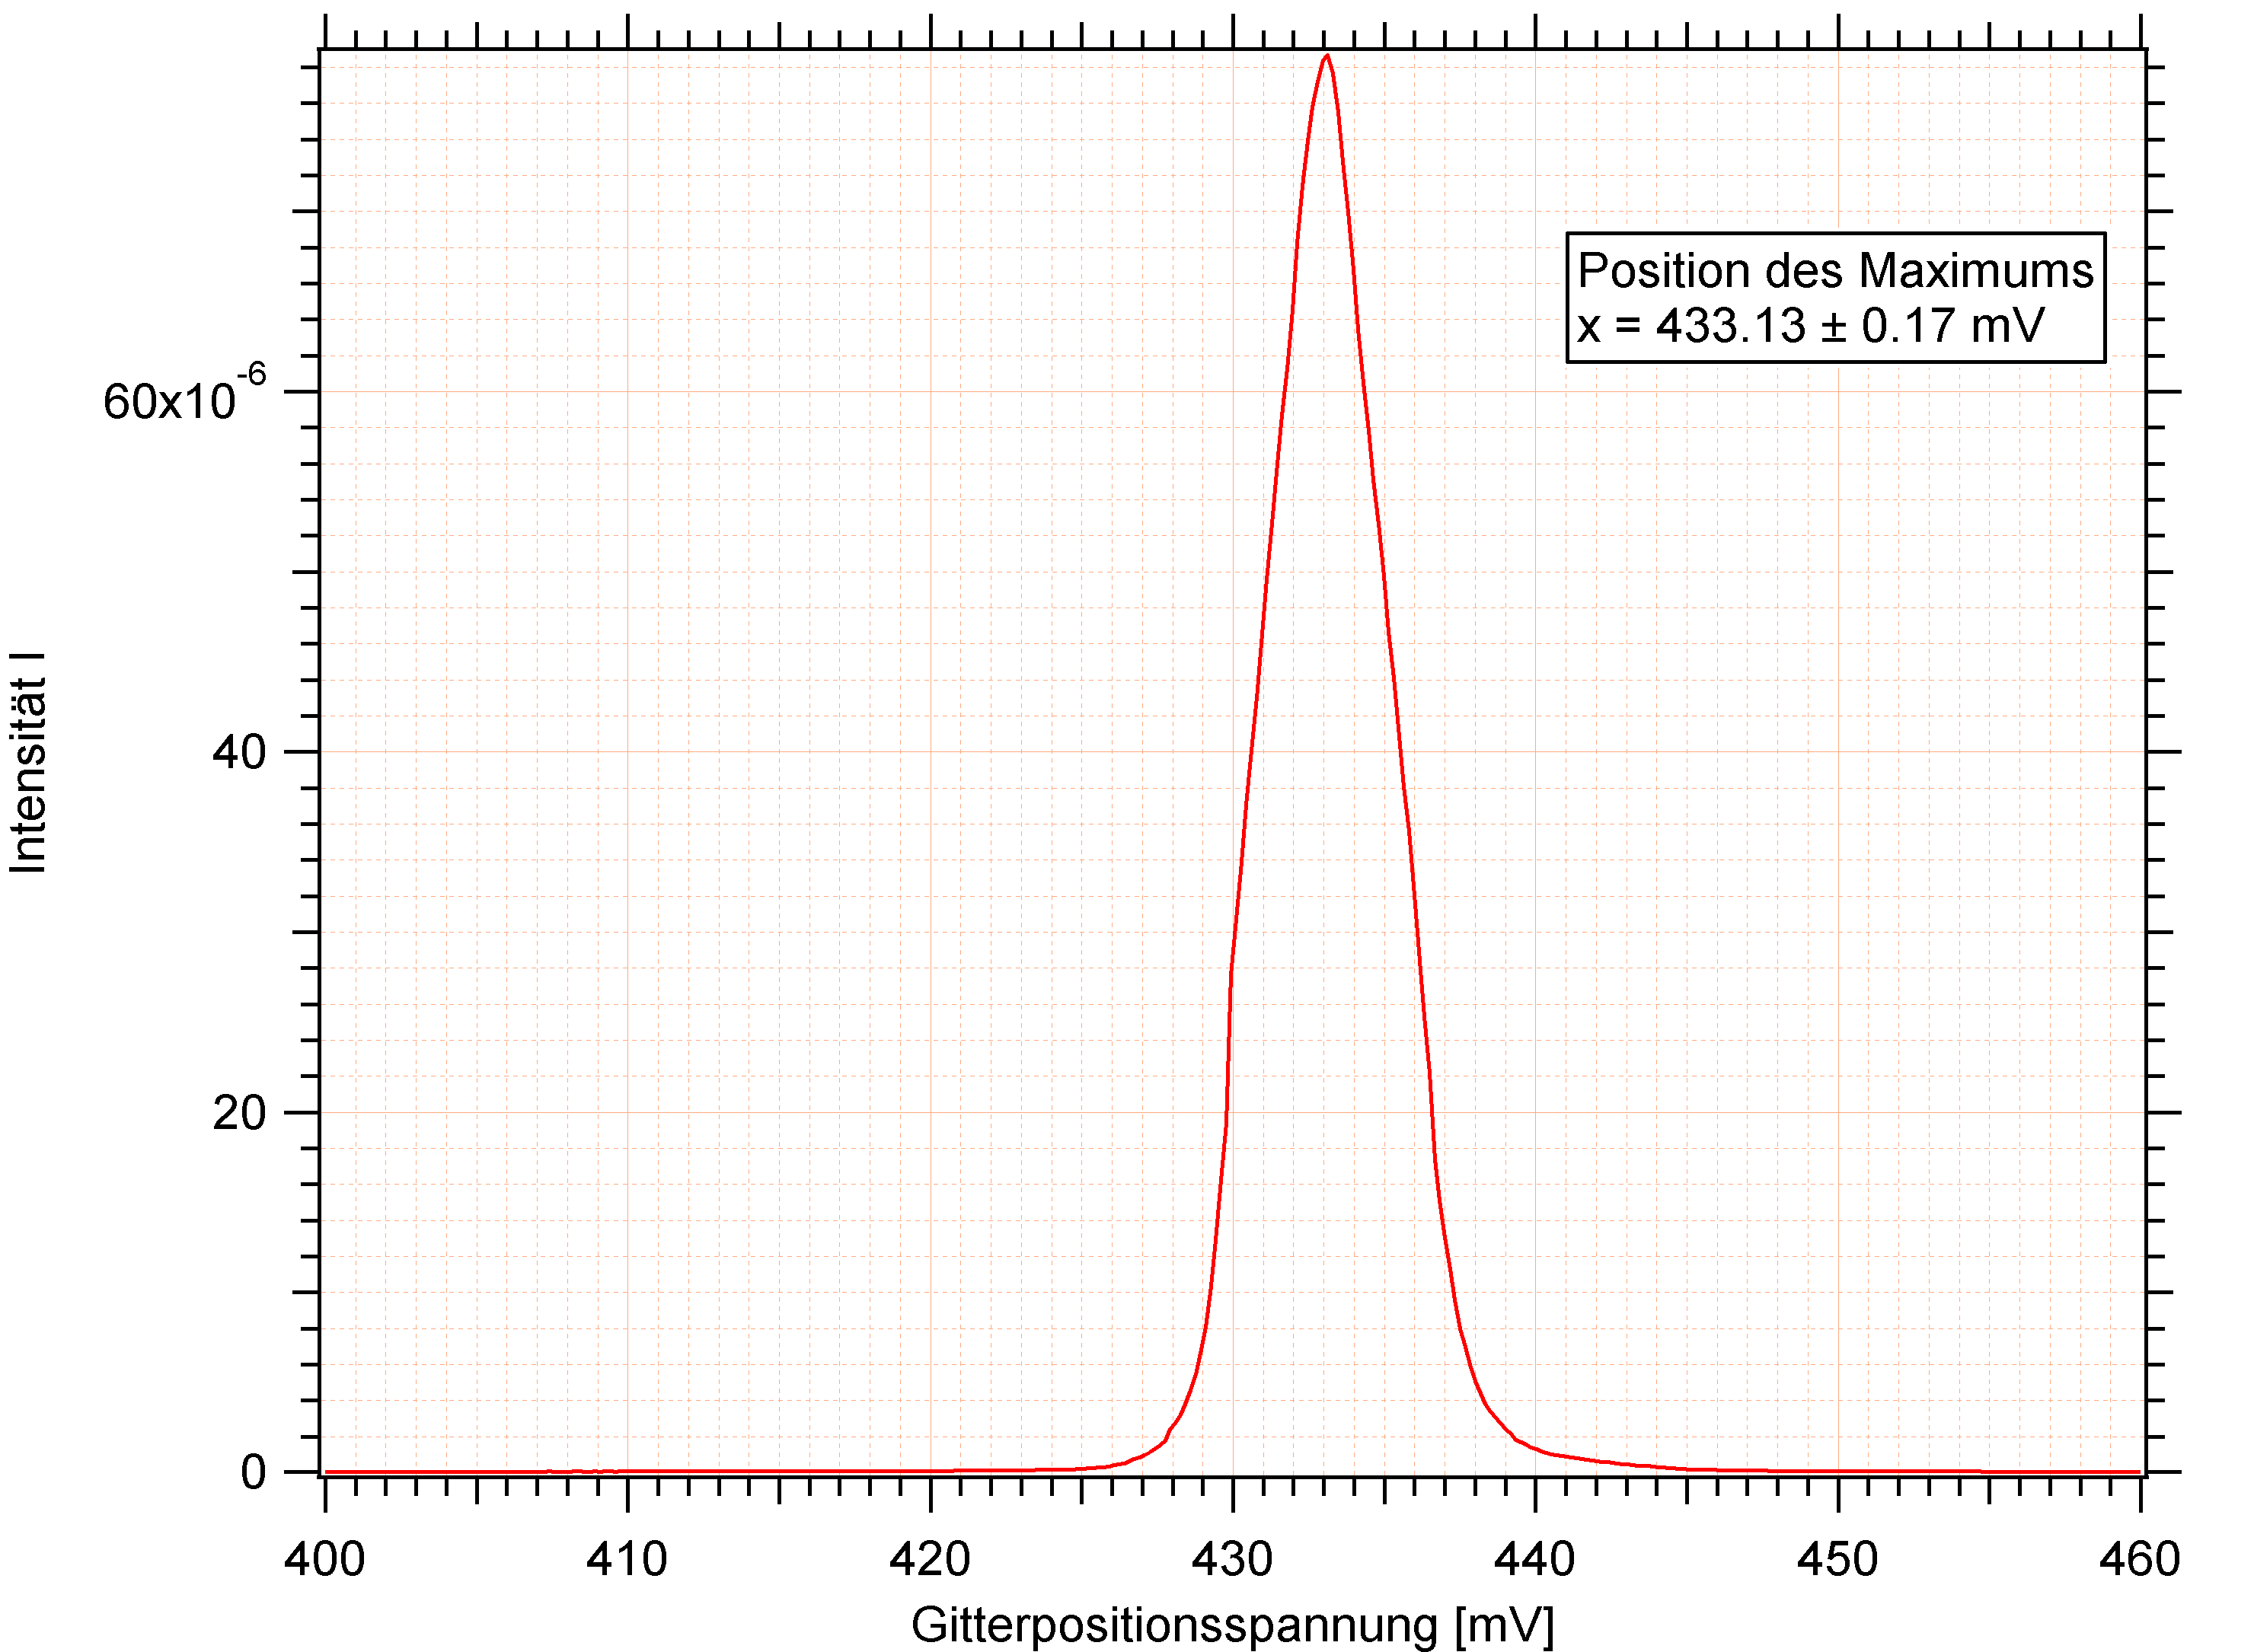
\includegraphics[width=\columnwidth]{Bilder/Graph1.png}
	\end{minipage}
	
	
	\caption{Emissionsspektrum einer Natriumdampflampe bei der nullten Ordnung. Das Spektrum wurde durch Aufspaltung des Lichts mit einem Czerny-Turner-Monochromator aufgenommen, wobei die Detektion mit einem Photomultiplier erfolgte. Die Daten wurden mittels Igor Pro 6.37 ausgewertet.}
	

	\label{Null}
\end{figure}
%%%%%%%%%%%%%%%%%%%%%%%%%%%	
\begin{figure}[H]
	\centering	
	\begin{minipage}{1\textwidth}
	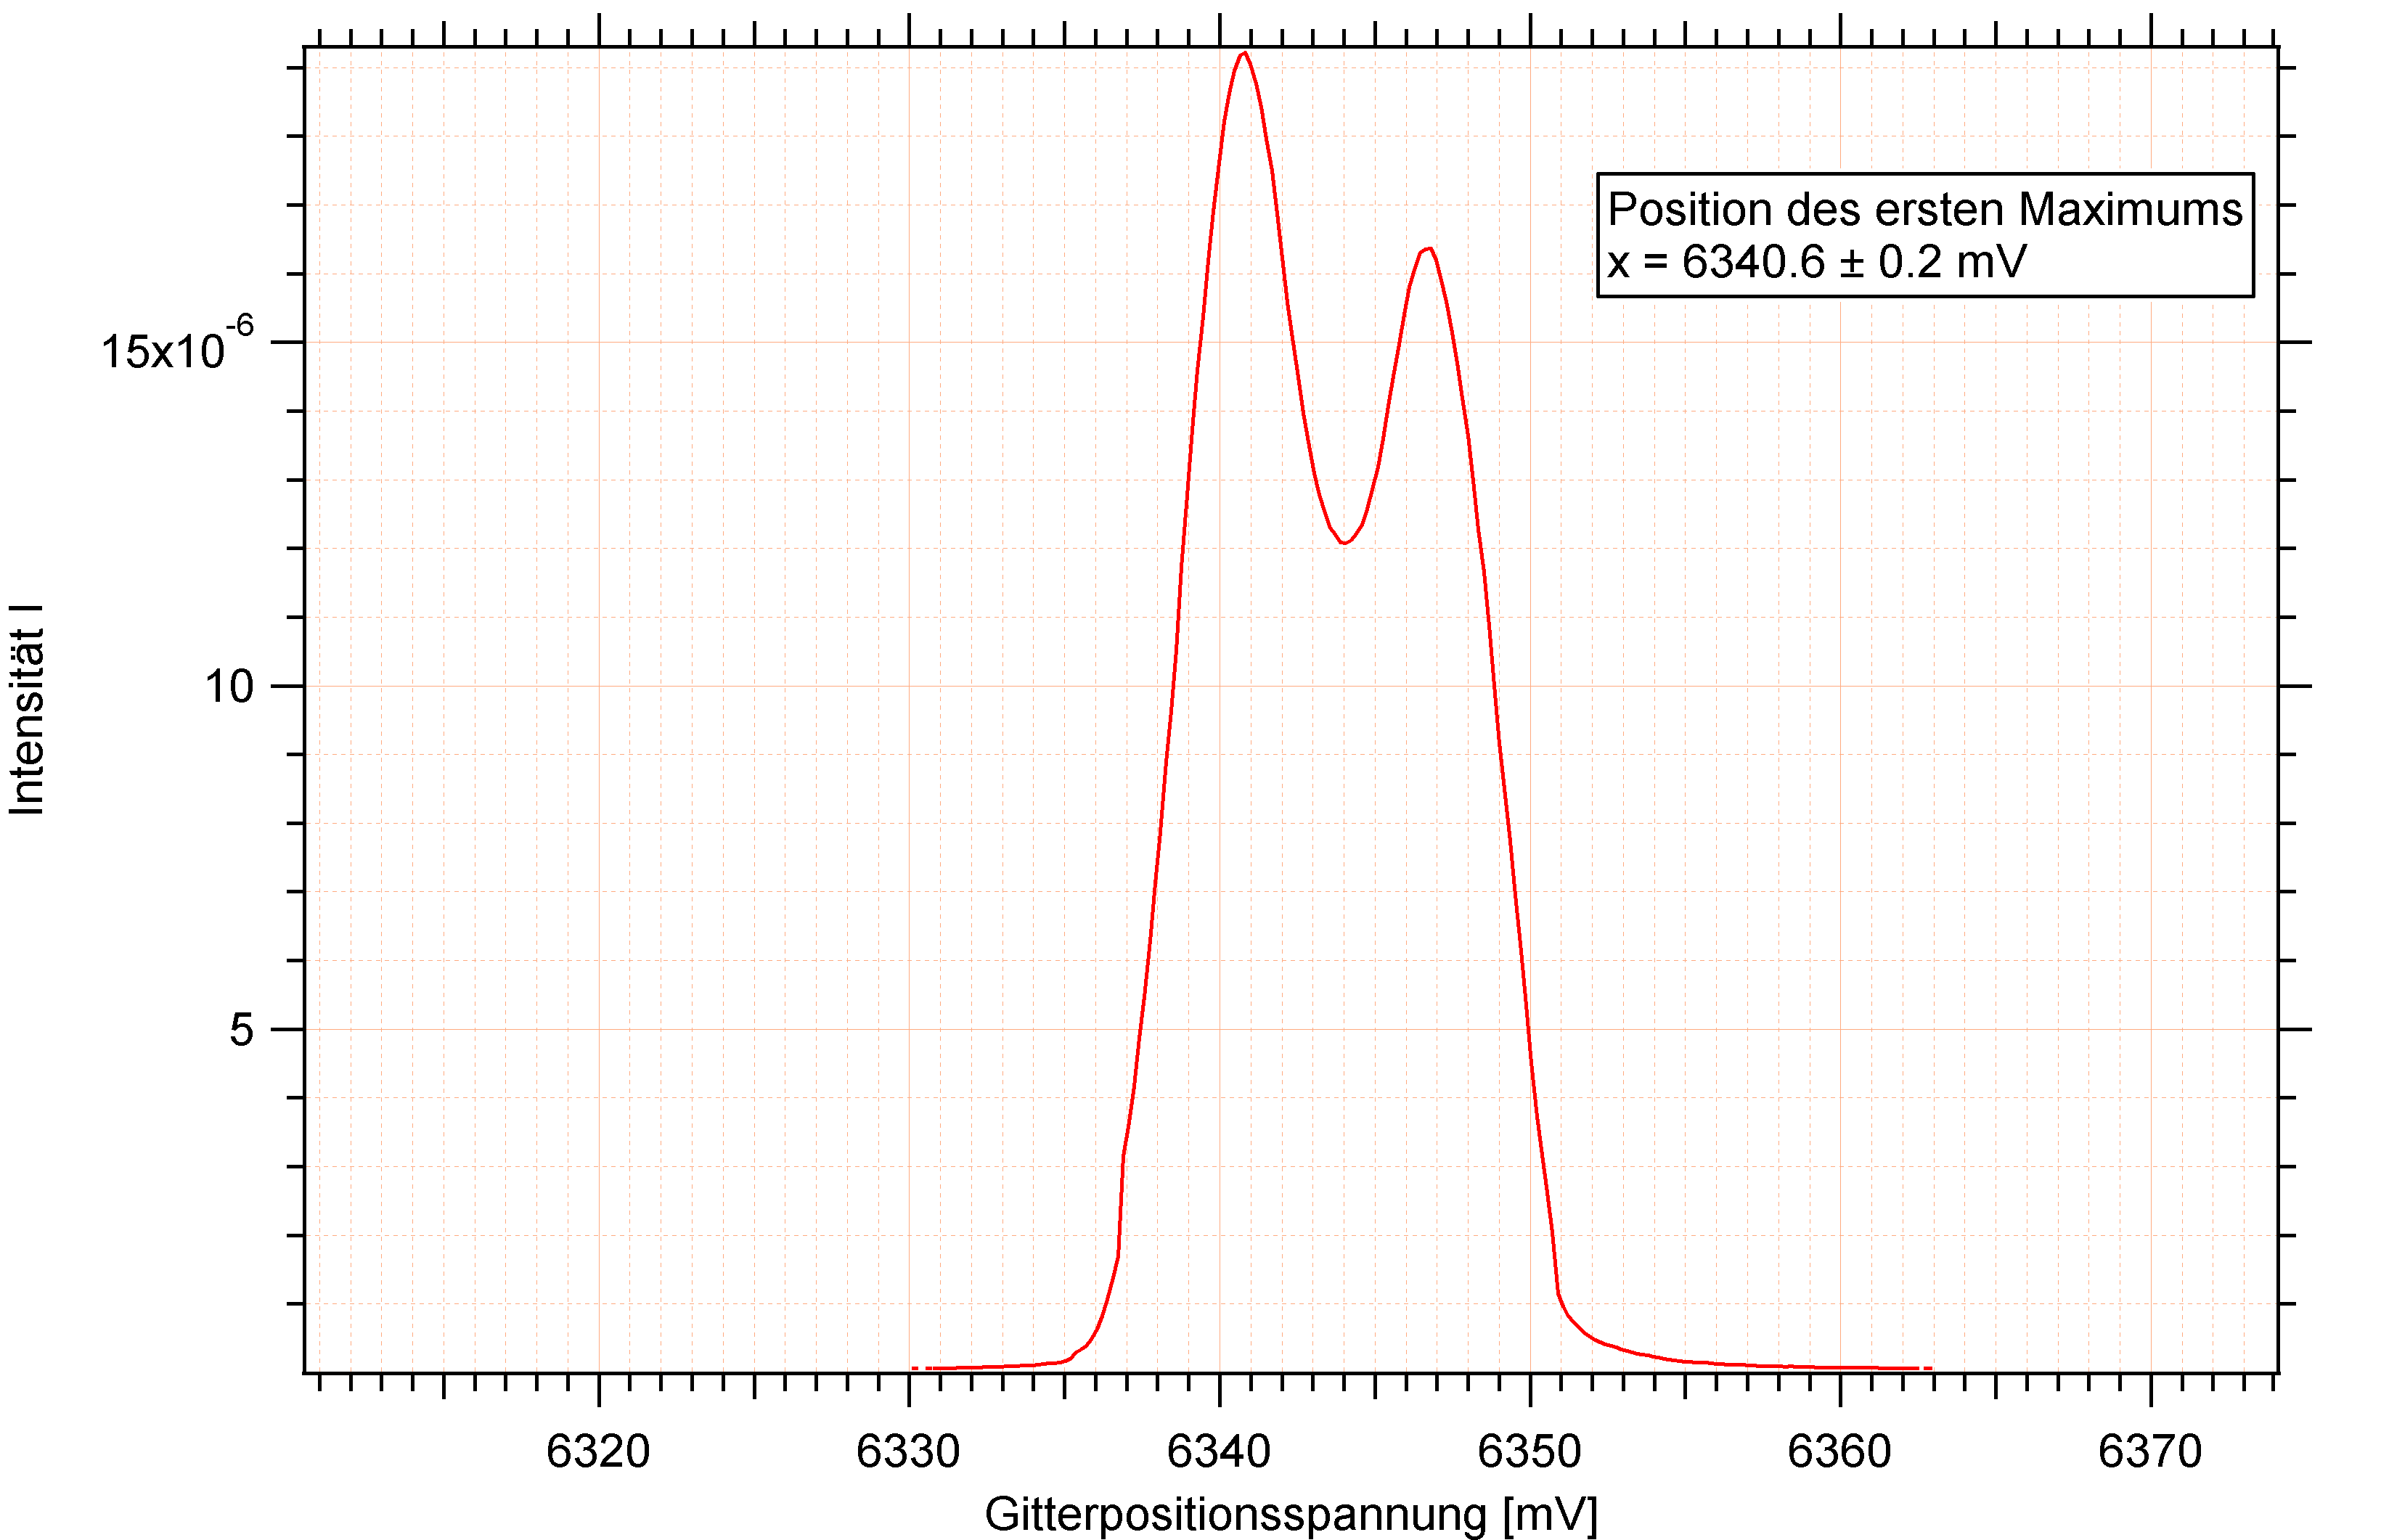
\includegraphics[width=\columnwidth]{Bilder/Graph2.png}
	\end{minipage}
	
	
	\caption{Emissionsspektrum einer Natriumdampflampe bei der ersten Ordnung. Das Spektrum wurde durch Aufspaltung des Lichts mit einem Czerny-Turner-Monochromator aufgenommen, wobei die Detektion mit einem Photomultiplier erfolgte. Die Daten wurden mittels Igor Pro 6.37 ausgewertet. Der größere Peak entspricht der Natrium-D-2 Linie bei 588.995~\si{nm}.}
	
	
	\label{Eins}
\end{figure}



Da die Wellenlängen der Natrium-D-Linien hinreichend bekannt sind $^{[1]}$, ist es möglich aus der Spannung, die mit der Position des Gitters korreliert, die Änderung der Wellenlänge pro Spannungsänderung zu berechnen.$^{[1]}$ Außerdem wurde durch die Spannung beim Peak der nullten Ordnung die Verschiebung der Wellenlängenskala zur Spannungsskala bestimmt.

\begin {equation}
\frac{dU}{d\lambda}=\frac{\Delta U}{\Delta\lambda}=\frac{6340.6~\si{mV} - 433.13~\si{mV}}{588.995~\si{nm}}=10.03~\si{\frac{mV}{nm}} 
\end {equation}

Der Fehler hierbei berechnet sich additiv gemäß der folgenden Gleichung:

\begin {equation}
\Delta\left(\frac{\Delta U}{\Delta \lambda}\right) = \Delta U_1 + \Delta U_2 = 0.2~\si{mV}+0.17~\si{mV}=0.37~\si{mV}
\end{equation}

Auf dieser Grundlage wurde das Emissionsspektrum \ref{Bunsen} einer rauschenden Bunsenbrennerflamme aufgenommen, welche mit Butan betrieben wurde. In dem untersuchte Energiebereich, kann die Relaxation des elektronisch angeregten $C_2$ beobachtet werden.



\begin{figure}[H]
	\centering	
	\begin{minipage}{1\textwidth}
	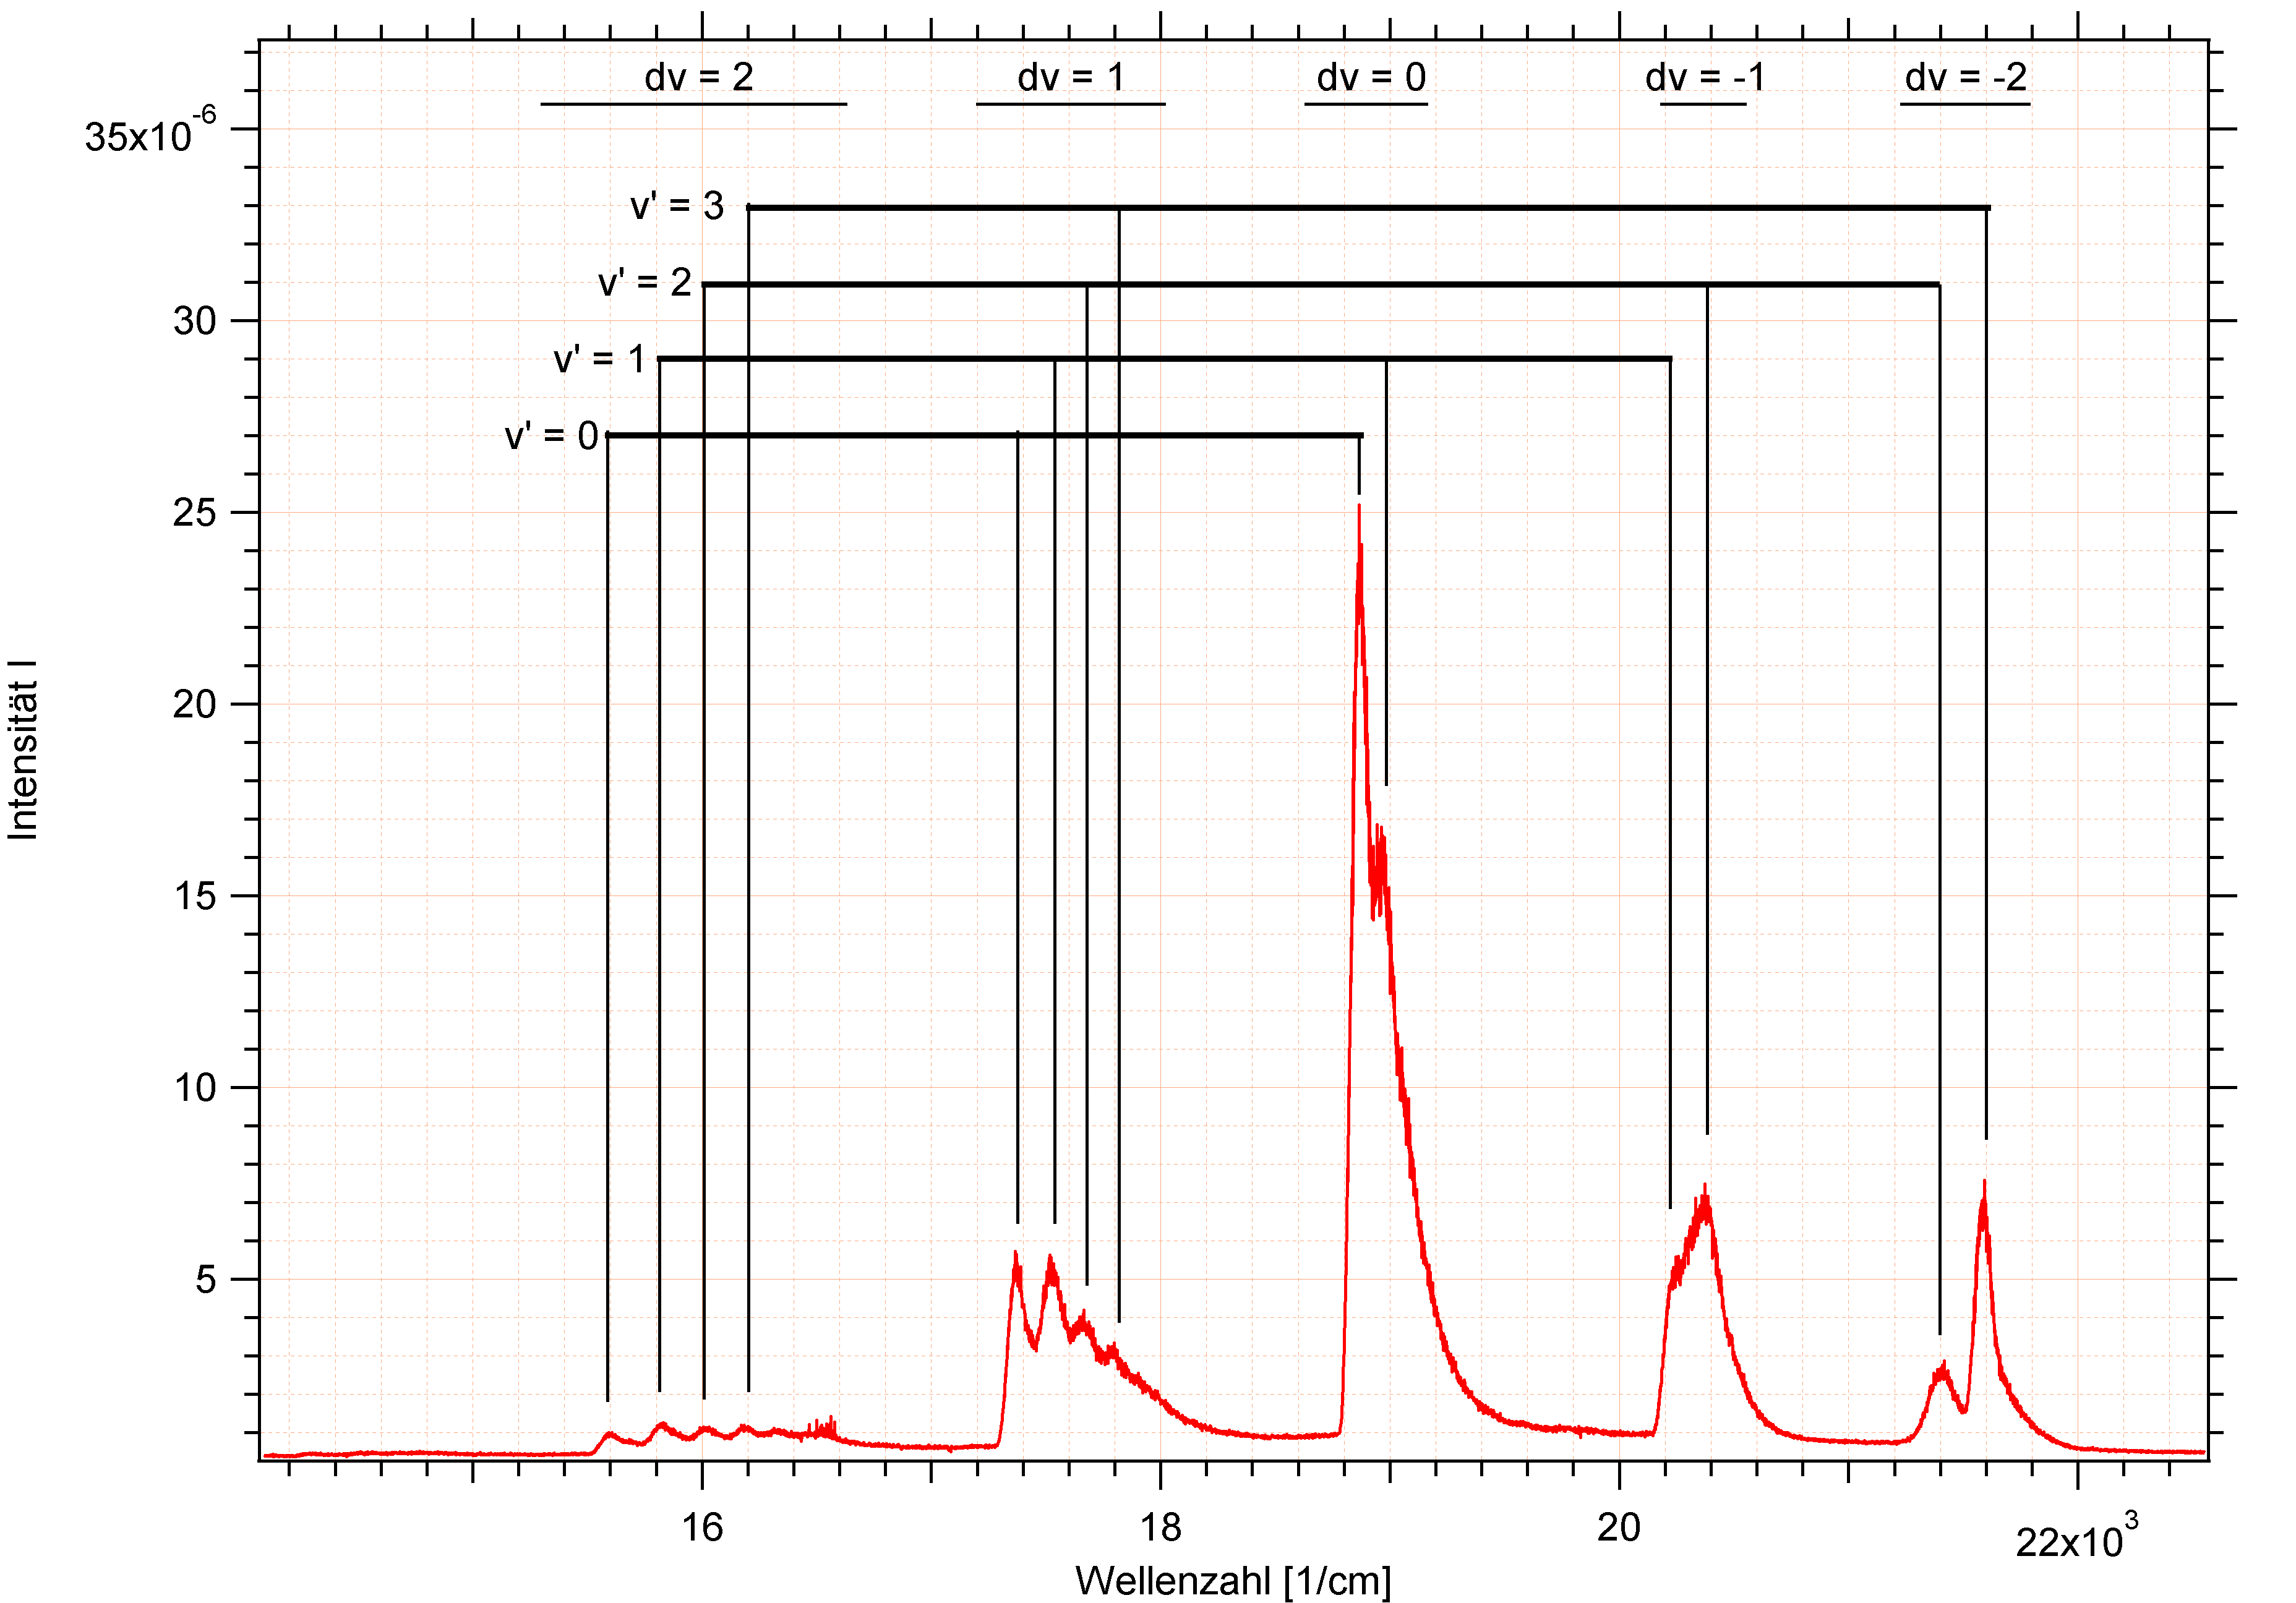
\includegraphics[width=\columnwidth]{Bilder/Graph3.png}
	\end{minipage}
	
	
	\caption{Emissionsspektrum der Bunsenbrennerflamme. Das Spektrum wurde durch Aufspaltung des Lichts mit einem Czerny-Turner-Monochromator aufgenommen, wobei die Detektion mit einem Photomultiplier erfolgte. Die Daten wurden mittels Igor Pro 6.37 ausgewertet. Die Peaks sind den entsprechenden Übergängen zugeordnet.}
	

	\label{Bunsen}
\end{figure}

Durch die Zuornung  markanter Banden war es möglich mit einer, durch den Praktikumsleiter bereitgestellten, vorimplementierten Routine die gesuchten Konstanten zu finden. Diese sind  $\nu_e$, die harmonischen Schwingungskonstanten und die Anharmonizitätskonstanten des Grund,sowie des angeregten Zustandes, welche in Tabelle  \ref{tab1} zusammengefasst sind.


\begin{table}[H]

 
 \caption{Zusammenfassung der Ergebnisse des Fits zur Bestimmung der Konstanten. Alle Werte sind in $\si{cm}^{-1}$ angegeben.}
\begin{tabular}{C{0.3\linewidth}|C{0.3\linewidth}C{0.3\linewidth}}

 
 Konstante &  Messwert &  Literatur $^{[1]}$\\
  \hline \addlinespace[1ex] 
$\nu_e$ & $18813 \pm 5.45$ & \\
$\omega'_e$ & $1544.7 \pm9.92$ & $1641.35$ \\
$\omega'_e x'_e$ & $25.5 \pm 3.0$ &  $11.67$ \\
$\omega''_e$ & $1649.2 \pm 9.92$ & $1788.22$ \\
$\omega''_e x''_e$ & $28.75 \pm 4.18$ & $16.440$ \\
 
   
 \end{tabular}
 \label{tab1}
 \end{table}


Beim Vergleich der angepassten Werte mit den Literaturwerten ist ersichtlich dass die ermittelten Werte nicht verträglich sind, jedoch die Größenordnung sehr gut gefunden wurde. 

Aus diesen Werten wurde nun mit Hilfe von Gleichung \ref{1} die Übergangswellenzahlen weiterer Übergänge berechnet, welche in Tabelle \ref{tab2} dargestellt sind.



\begin{table}[H]
 
\caption{Deslandres-Tabelle der beobachteten Übergänge in $\si{cm}^{-1}$. Die Werte gehen aus der Berechnung mit Gleichung \ref{1} hervor}
\begin{tabular}{L{0.1\linewidth}|L{0.1\linewidth}L{0.1\linewidth}L{0.1\linewidth}L{0.1\linewidth}L{0.1\linewidth}L{0.1\linewidth}L{0.1\linewidth}}

 
v'/v'' & 0 & 1 & 2 & 3 & 4 & 5 & 6\\
\hline \addlinespace[1ex]
$0$ & $18860 \pm 20$ & $17370 \pm35$ & $15930 \pm 55 $ &  $ $ & $ $ & $ $ &  \\
$1$ & $20460 \pm 35$ & $18960 \pm 50$ & $17520 \pm 70 $ & $16150 \pm 100$ & $ $ & $ $ &  \\
$2$ & $21990$ & $20496$ & $19053$ & $17662$ & $16321$ & $ $ &  \\
$3$ & $ $& $21973$ & & & $17798$ & $16508$ & \\
$4$ & $ $ & $ $ & $ $ & $ $ & $ $ & $ $ & $16689$ \\
 
   
 \end{tabular}
 \label{tab2}
 \end{table}






\end{document}